\chapter{Introduction générale}% 5 à 10 pages
%\addstarredchapter{Introduction générale}
\minitoc
\newpage
\rule{\linewdith}{1pt}
\section{Contexte et motivations}

\subsection{Contexte de travail}%LIMOS,IMOBS3, PAVIN
Ce travail de thèse a été réalisé au sein du LIMOS (Laboratoire d'Informatique, de Modélisation et d'Optimisation des Systèmes). Le LIMOS est une Unité Mixte de Recherche (UMR 6158) de l'Université Clermont Auvergne situé à Clermont-Ferrand en France.
Les résultats qu'on présentera dans ce rapport de recherche sont le fruit d'une collaboration entre l'axe MAAD et l'axe ODPS qui font partie des trois principaux axes de recherche du LIMOS. Ces axes sont respectivement l'axe Modèles et Algorithmes de l'Aide à la Décision (MAAD), l'axe Outils Décisionnels pour la Production et les Services (ODPS) et l'axe  Systèmes d'Information et de Communication (SIC). Le positionnement scientifique de chacun de ces axes est le suivant :
\begin{itemize}[label=$\square$]
	
	
	\item Les chercheurs de MAAD s'intéressent à la résolution mathématique et algorithmique de problèmes d'optimisation \cite{wilde1967foundations} en Recherche Opérationnelle. Ils explorent plusieurs approches en particulier les algorithmes d'approximation (algorithmes qui produisent en temps polynomial des solutions dont on peut garantir la qualité par rapport à la solution optimale) et les méthodes polyédrales (approches qui consistent à ramener chaque problème à la résolution d'un programme linéaire). 


	\item Les chercheurs d'ODPS s'occupent de la modélisation de systèmes complexes et de l'implémentation des méthodes aidant à la prise de décisions. La plupart du temps, ils identifient dans un premier temps des problématiques nouvelles et par la suite conçoivent des méthodes d'optimisation capables de les traiter efficacement. 
	
	\item Les chercheurs de SIC s'intéressent à la collecte (à travers par exemple des mécanismes de communication sans fil), la gestion et l'analyse de grande masse de données en utilisant des techniques de fouille de données et d'apprentissage automatique.
\end{itemize}

Le LIMOS est membre du Laboratoire d'Excellence pour la Mobilité Innovante des personnes, des biens et des machines dont l'acronyme est Labex IMobS3.
% et est cofinancé par le Labex IMObS3 et la région Auvergne.
%Ce travail de thèse à été réalisé au sein du Laboratoire d'Informatique, de Modélisation et d'Optimisation des Systèmes (LIMOS) à Clermont-Ferrand en France.
% Le LIMOS est une Unité Mixte de Recherche (UMR 6158) en informatique, et plus généralement en Sciences et Technologies de l'Information et de la Communication (STIC). 
 %Le LIMOS est principalement rattaché à l'Institut des Sciences de l'Information et de leurs Interactions (INS2I) du CNRS, et de façon secondaire à l'Institut des Sciences de l'Ingénierie et des Systèmes (INSIS). Il a pour tutelles académiques l'Université Blaise Pascal (UBP)- Clermont-Ferrand II, l'Université d'Auvergne (UdA)-Clermont-Ferrand I, et l'Ecole Nationale Supérieure des Mines de Saint-Etienne (EMSE), et comme établissement partenaire l'Institut Français de Mécanique Avancée (IFMA).  
% Il est membre associé de la fédération MOD-MAD (MODélisation Mathématique et Aide à la Décision, FED 4169) portée par Université Jean Monnet de Saint-Etienne.
 % Le positionnement scientifique du LIMOS est centré autour de l'Informatique, la Modélisation et l'Optimisation des Systèmes Organisationnels et Vivants. Les principaux thèmes de recherche développés au sein du laboratoire sont : optimisation combinatoire et continue ; recherche opérationnelle, Systèmes de production ; Logistique ; algorithmique des graphes et des treillis ; images et apprentissage ; modélisation et simulation ; grandes masses de données ; fouille de données ; interopérabilité des systèmes d'information ; réseaux de Capteurs et confiance numérique.
Le Labex IMobS3 a cofinancé cette thèse à hauteur d'environ $1/3$ du financement total et a utilisé un budget adossé sur des financements provenant d'une aide de l'état et gérés par l'Agence Nationale de la Recherche (ANR) au titre du programme Investissements d'Avenir. Le Laboratoire d'Excellence IMobS3 conçoit des systèmes respectueux de l'environnement pour une mobilité innovante des personnes (par exemple l'équipement de fauteuils pour personnes à mobilité réduite, et l'équipement de cannes blanches pour les personnes malvoyantes), des biens (par exemple le routage de véhicules autonomes pour le transport de marchandise) et des machines (par exemple le routage de drones). De plus, ils étudient les interactions entre des systèmes de mobilité innovante et leur environnent, ainsi que l'impact économique lié à la mise en place de tels systèmes, et l'impact sur l'Homme ou sur la Société comme par exemple les niveaux de prix d'accès au système proposés à l'utilisateur. Le but est de satisfaire les besoins des utilisateurs et d'augmenter la capacité de service en automatisant le plus possible certains travaux. Un autre axe d'étude du Labex IMobS3 est la recherche de procédés de production d'énergie renouvelable pour alimenter les systèmes de mobilité innovante. Une énergie est dite renouvelable lorsqu'elle provient de sources que la nature renouvelle en permanence.
Les systèmes de mobilité innovante conçus sont testés au sein de plateformes expérimentales appelées PAVIN.

  On a travaillé dans le cadre de ce projet, avec des chercheurs de PAVIN qui nous ont renseigné sur les mécanismes de fabrication des énergies renouvelables. Il existe trois plateformes PAVIN : la plateforme \textbf{PAVIN VU « Véhicule Urbains »} (Voir figure	\ref{pavin}), la plateforme \textbf{PAVIN VMN « Véhicule en Milieu Naturel »} (Voir figure	\ref{pavin_vmn}) et la plateforme \textbf{PAVIN BP « Brouillard et Pluie »} (Voir figure	\ref{pavin_bp}). Le rôle de chaque plateforme est le suivant :
  \begin{itemize}[label=$\square$]
 
  \item  La plateforme \textbf{PAVIN VU} simule une mini-ville disposant de différents véhicules électriques et travaille sur les procédés permettant d'accroître le degré d'autonomie de ces derniers.  Ce site expérimental original situé à Clermont-Ferrand (France), a été conçu pour le déplacement de véhicules autonomes. 
  \item La plateforme \textbf{PAVIN VMN} se trouve sur le site de Montoldre de l'Institut National de Recherche en Sciences et Technologies pour l'Environnement et l'Agriculture (IRSTEA) dans l'Allier. Ce site de 70 hectares permet de faire évoluer divers véhicules à haute vitesse.
  \item  La plateforme \textbf{PAVIN BP} du Centre d'Etudes et d'Expertise sur les Risques, l'Environnement, la Mobilité et l'Aménagement (CEREMA) est composée d'une part d'un tunnel permettant de simuler des conditions atmosphériques dégradées tant pour le brouillard que la pluie (plateforme unique au plan national) et d'autre part d'un dispositif mobile pouvant être déployé sur \textbf{PAVIN VU} et \textbf{PAVIN VMN}. Cette plateforme se situe à Clermont-Ferrand.
\end{itemize}
Toutes ces plateformes se situent dans la région AURA, Auvergne-Rhône-Alpes.

Finalement, le FEDER-Region Auvergne a cofinancé cette thèse à hauteur d'environ $2/3$ du financement total et a utilisé une aide de l'Union Européenne via les Fonds Européen de Développement Régional (FEDER-Région Auvergne). %L'AURA est l'une des régions françaises les plus productrices d'énergie.
 
En Auvergne, on distingue trois types de filières de production d'énergie : 
\begin{itemize}[label=$\square$]
	
	\item La filière classique qui regroupe les centrales nucléaires et thermiques. 
		\item La filière d'énergie renouvelable thermique (bois énergie, pompes à chaleur, solaire, valorisation thermique des déchets et du biogaz, etc). 
			\item La filière d'énergie renouvelable électrique (hydraulique, éolien, photovoltaïque, valorisation électrique des déchets et du biogaz, etc). 
\end{itemize}
Notre projet de thèse fait partie d'un vaste projet dont l'objectif est la vulgarisation de l'utilisation des énergies renouvelables, plus précisément de l'\textbf{hydrogène} solaire.

 %La spécificité d'IMobS3 repose sur la mise en place de solutions de mobilité durable via des approches coopératives couplant des disciplines diverses.
 %Le LabEx IMobS3 fait partie de cinq établissements clermontois (l'Université Clermont Auvergne - porteur du projet, l'école d'ingénieur SIGMA Clermont, le CNRS, l'Irstea et le Cerema). Il s'appuie sur les compétences de plusieurs laboratoires (ACTé, DLCF-CEREMA, LAPSCO, LIMOS, LMBP, ICCF, Institut Pascal, TSCF-IRSTEA) placés sous la tutelle de ces établissements souvent sous la forme d'unités mixte de recherche.
 %En février 2017, la communauté universitaire Clermontoise a obtenu le label I-Site « Initiatives – Science - Innovation - Territoires - Economie » grâce au projet CAP 20-25 qui vise à structurer le site universitaire en s'appuyant sur les succès acquis lors du premier appel à projet investissements d'avenir.
 %Le LabEx IMobS3 s'avère être la pierre angulaire du Challenge « Systèmes et services pour la production et les transports ».
 %La spécificité d'IMobS3 repose sur la mise en place de solutions de mobilité durable via des approches coopératives couplant des disciplines diverses et s'articulant autour du triptyque « Recherche – Formation – Valorisation  ».
 %Le but de ce challenge est d'étudier la façon dont de nouveaux services ou systèmes industriels susceptibles de mettre en œuvre des objets dédiés à la mobilité de personnes, biens ou machines devraient être conçus, dimensionnés, tarifés et pilotés de façon à s'intégrer dans leur environnement économique, juridique et sociétal. De fait, l'accent est mis principalement sur l'Intelligence Computationnelle à même de contribuer au design et management de ces services et systèmes. De plus, les aspects liés à l'Economie de la Mobilité ou à la relation de ces systèmes à l'Homme ou à la Société ne sont pas non plus ignorés.
 
 %Ainsi, nous nous concentrons sur la façon dont une certaine forme d'Intelligence Computationnelle peut être introduite aux fins d'accroitre la capacité de services et systèmes émergents, mettant en jeu des formes innovantes de mobilité, à satisfaire les besoins des utilisateurs tout en maintenant un équilibre économique.

%  L'étude de ces systèmes doit amener les chercheurs à concevoir des modèles numériques, des algorithmes décisionnels, des modules de traitement des données et des architectures d'acquisition, de communication et de supervision, à même de faciliter, pour ces systèmes : le dimensionnement, la planification, la supervision, le pilotage, etc.
  
% Dimensionner et planifier efficacement un système suppose la mise au point de modèles agrégés d'optimisation, statiques ou dynamiques, cohérents avec les modèles descriptifs de simulation, qui proposent différents scénarii organisationnels : tournée, périodicité des opérations de maintenance ou de redéploiement, dimensionnement des ressources humaines et matérielles, protocole de dialogue système/utilisateur. L'impact de ce processus sur la qualité de service (QoS) et la viabilité économique du système peut être décisif.
 
% Dans le cas de systèmes à haut niveau de réactivité, qui mettent en jeu des véhicules ou objets mobiles dotés de dispositifs embarqués intelligents, il s'agit alors de spécifier à la fois l'architecture qui permet tant l'acquisition et la transmission de l'information par les différents composants du systèmes que le dialogue avec l'utilisateur, et les mécanismes de décision (allocation des ressources aux demandes, gestion des perturbations, routage, etc) qui permettent au système de réagir en temps réel aux sollicitations.
 
 
 
 %\subsection{Energies renouvelables}


 %Plusieurs acteurs travaillent à la résolution de cette difficulté, à l'instar : du Labex IMobS3 « \textit{Innovative MOBility: Smart and Sustainable Solutions} », de PAVIN « Plateforme Auvergnate pour les Véhicule INtelligents », de la région AURA « AUvergne-Rhône-Alpes », de l'Agence Internationale pour les Energies Renouvelables abrégé IRENA « \textit{International Renewable Energy Agency} », etc. 
 %Actuellement en France, l'hydraulique est la première source d'énergie « propre ». 
    
%  Il existe un organisme appelé IRENA  dont l'objectif est de servir de centre mondial de coopération pour l'énergie renouvelable et d'échange d'informations entre ses 150 membres (149 États et l'Union Européenne).L'IRENA soutient les États dans leur transition vers un avenir énergétique durable et sert de principale plateforme pour la coopération internationale. Il est un référentiel de connaissances politiques, technologiques, et financières sur les énergies renouvelables. L'IRENA encourage l'adoption généralisée et l'utilisation durable de toutes les formes d'énergies renouvelables, y compris la bioénergie, l'énergie géothermique, l'hydroélectricité, les énergies marines, les énergies solaires et l'énergie éolienne dans la poursuite du développement durable et de la croissance économique faible en carbone.
 



  \subsection{Hydrogène}
  
 
 L'intérêt pour l'hydrogène vient du fait qu'à ce jour, les principales sources d'énergie sont les ressources fossiles par exemple le pétrole, le gaz naturel et le charbon. Ces ressources fossiles mettent des millions d'années (environ 250 millions) à se former, elles sont très polluantes, elles sont présentes en quantités limitées et se renouvellent beaucoup plus lentement que nous les utilisons. En France, la filière hydrogène n'est pas encore très développée, mais la société Air liquide et la société  MYRTE basée en Corse fabriquent déjà l'hydrogène. 
  \begin{figure}[H]
  	\centerline{
  		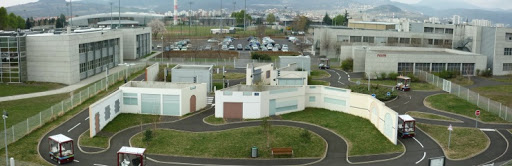
\includegraphics[height=5cm]{images_these/pavin.jpg}}
  	\caption[Plateforme PAVIN « Véhicule Urbains »]{ Plateforme \textbf{PAVIN « Véhicule Urbains »} \cite{plateforme}.}
  	\label{pavin}
  \end{figure}
  \begin{figure}[H]
  	\centerline{
  		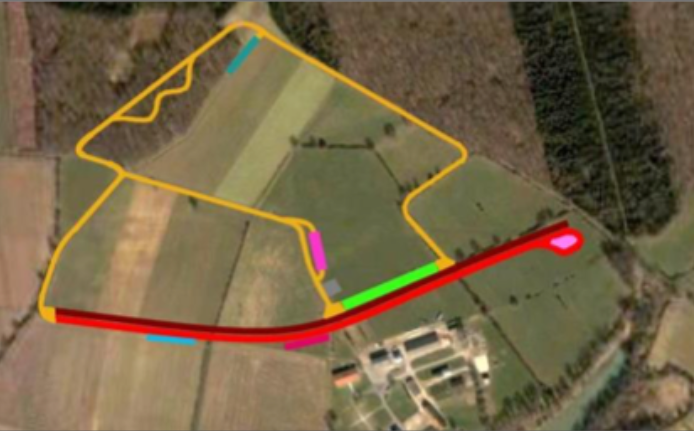
\includegraphics[height=7cm]{images_these/pavin_VMN.png}}
  	\caption[Plateforme PAVIN VMN « Véhicule en Milieu Naturel »]{ Plateforme \textbf{PAVIN VMN « Véhicule en Milieu Naturel »} \cite{plateforme}.}
  	\label{pavin_vmn}
  \end{figure}
  \begin{figure}[H]
  	\centerline{
  		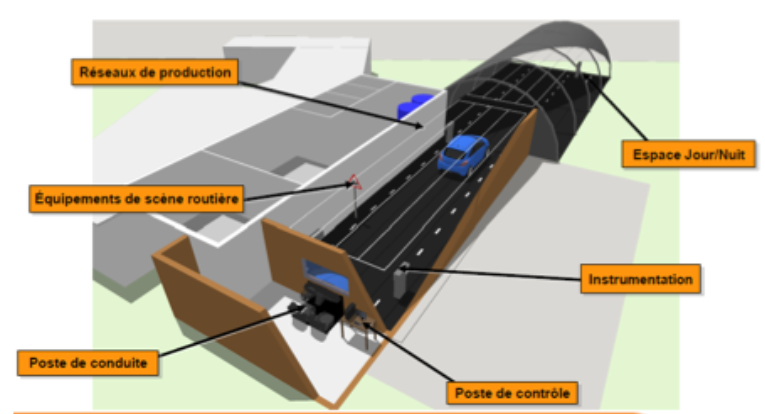
\includegraphics[height=7cm]{images_these/pavin_BP.png}}
  	\caption[Plateforme PAVIN BP « Brouillard et Pluie »]{ Plateforme \textbf{PAVIN BP « Brouillard et Pluie »} \cite{plateforme}.}
  	\label{pavin_bp}
  \end{figure}
 Actuellement, il existe trois procédés de fabrication de l'hydrogène : 
 \begin{itemize}[label=$\square$]
 	%la transformation de l'eau, du soleil et un catalyseur consiste à diviser les rayons solaires en deux parties les rayons visible et les rayons invisible puis, à utiliser ces rayons visible pour casser la molécule d'eau afin d'obtenir un gaz contenant de l'hydrogène. Ensuite à l'aide d'une énergie mécanique, nous allons extraire l'hydrogène de ce gaz. 
 	\item L'hydrogène peut être produite par électrolyse de l'eau ($H_2O$). L'électrolyse de l'eau ($H_2O$) consiste à casser la molécule d'eau à l'aide de l'électricité afin d'obtenir de l'hydrogène pure (technique utilisée dans les boosters des fusées Ariane). Pour le faire, on a besoin d'une photo-catalyse et d'un catalyseur. On utilise l'électrolyse alcaline ou l'électrolyse basique dont la différence se trouve au niveau de l'acidité de l'eau. La quantité d'hydrogène produite est $100$ $ m^3/heure$. Cette technique est utilisée par MYRTE.
 	\item L'hydrogène peut être produite par vaporeformage du méthane ($CH_4$). Le vaporeformage du méthane ($CH_4$) consiste à produire de l'hydrogène en utilisant le méthane, une source de chaleur et de l'eau, mais l'énergie produite n'est pas renouvelable. Par contre la quantité d'hydrogène fabriquée est énorme ($100.000 $ $ m^3/heure$). Cette technique est utilisée par la société Air liquide. L'inconvénient de cette méthode est qu'elle produit beaucoup de $CO_2$.
 
 	\item L'hydrogène peut être produite par photolyse de l'eau. Lors de la photolyse, l'énergie de la lumière solaire provoque la cassure des molécules d'eau. On utilise des cellules photo-électrochimiques (PEC), constituées d'électrodes photosensibles et plongées dans l'eau. La lumière absorbée génère des électrons (négatifs) et des charges positives formées par des manques d'électrons appelés trous. En présence de ces paires électrons-trous, les molécules d'eau subissent une réaction d'oxydo-réduction. Hydrogène et oxygène partent chacun de leur côté sous forme gazeuse, $H_2$ et $O_2$. Cette technique donne de meilleure quantité d'énergie (beaucoup de $H_2$) que l'électrolyse de l'eau mais il faudrait une grande surface pour pouvoir capter du soleil. Cette technique est à un stade expérimental et a été le projet de thèse en Génie des procédes de \textbf{Victor Gattepaille} sous la direction de \textbf{Jean francois Cornet}, en partenariat avec Institut Pascal de Novembre 2017 à Janvier 2021.
 \end{itemize}
 
 \begin{table}[H]
 	\begin{center}
 		\begin{tabular}{|m{3.5cm}|m{3.5cm}|m{3.5cm}|m{3.5cm}|}
 			
 			%|c
 			\hline
 			
 		\rowcolor{cyan}	\backslashbox{Caract.}{ Procédés}	&Photolyse   & Vaporeformage $CH_4$ & Electrolyse de l'eau \\
 			%Coût de la solution&  Optimum &
 			\hline
 			
 			Réalisé de nos jours	&	stade expérimental & oui  & oui \\
 			%2547 & 1443 &
 			\hline
 			
 			Nombre de $m^3$ par heure produite	&Supérieur à	$100 $ & $100.000 $  & $100 $ \\
 			% 1848 & 1443& 
 			\hline
 			
 			Difficultés	&Nécessite trop de soleil & Pas renouvelable  & Nécessite trop d'électricité \\
 			%2285 & 1443 &
 			\hline	
 			
 			Ingrédients	&	Eau, soleil & Méthane, eau, chaleur  & Eau, électricité  \\
 			%2285 & 1443 &
 			\hline	
 			Taux de pollution&Faible & Forte  & Celui pour produire l'électricité  \\
 			%2285 & 1443 &
 			\hline
 			
 			Société &En laboratoire & Air liquide  & MYRTE   \\
 			%2285 & 1443 &
 			\hline	
 		\end{tabular}
 		\caption{Comparaison entre les procédés de fabrication de l'hydrogène.}
 		\label{h}
 	\end{center}
 \end{table}
 Le tableau (\ref{h}) est un récapitulatif de l'étude comparative qu'on a faite entre les caractéristiques (appelées Caract.) des procédés de fabrication de l'hydrogène (appelés Procédés).
 
 
  Une énergie « propre » est une énergie qui produit une faible quantité de $CO_2$ lors de son utilisation et de sa fabrication. Concernant son utilisation, l'hydrogène est une énergie « propre » mais la façon dont on produit cet hydrogène n'est pas toujours « propre ». 
 L'un des avantages de l'hydrogène est sa bonne autonomie car par exemple les modèles de voiture à hydrogène aujourd'hui peuvent parcourir plus de 500  kilomètres. L'inconvénient de l'hydrogène est sa faible masse volumique. Pour conserver une grande quantité d'hydrogène on a ainsi besoin de très grands réservoirs. A cet effet, des réservoirs à 350 bar ont été conçus car en augmentant la pression dans un réservoir on diminue le volume de celui-ci accroissant la masse qu'il peut contenir.
 
 Il existe de nombreux cas d'applications de l'hydrogène, on a :
 \begin{itemize}[label=$\square$]
 
 \item Des applications  mobiles : l'hydrogène peut alimenter des véhicules équipés de moteurs à combustion fonctionnant au gaz. Par ailleurs, un réservoir d'hydrogène peut-être associé à une pile combustible pour améliorer l'autonomie de véhicules électriques. De plus, la mise en place de flottes captives (par exemple celles de La Poste) fonctionnant à l'hydrogène permet d'augmenter la productivité tout en diminuant les émissions de $CO_2$ sur le lieu d'utilisation. 
 Les principales applications concernent les flottes de chariots élévateurs d'entrepôts de logistique ou encore les flottes de véhicules de transport de bagages dans les aéroports. L'hydrogène peut aussi être utilisé comme carburant pour les fusées comme c'est la cas pour la Fusée Européenne Ariane 5.
 \item Des applications  stationnaires qui consistent à stocker de l'énergie dans des bâtiments en assurant une fourniture d'électricité et de chaleur grâce à la cogénération en produisant simultanément deux types d'énergie, et cela dans une même centrale. L'hydrogène permet une grande autonomie et est aussi particulièrement adapté à la fourniture d'énergie pour des équipements stationnaires éloignés du réseau (ou en attente de raccordement). C'est notamment le cas pour les antennes relais de téléphonie mobile.
 \item  Des applications industrielles : l'hydrogène est un composant chimique très employé dans l'industrie. De nombreuses applications industrielles l'utilisent pour produire différents matériaux.
 En électronique, l'hydrogène sert à la fabrication de composants. Il assure une excellente protection contre les impuretés.
 En chimie industrielle, l'hydrogène peut être associé à de l'azote pour fabriquer de l'ammoniac, une base des engrais. C'est un réactif qui entre dans la composition des fibres textiles comme le nylon et de diverses matières plastiques.
  Dans l'industrie du verre, l'hydrogène est indispensable à la fabrication du verre plat utilisé notamment pour les écrans plats.
 L'hydrogène est employé en métallurgie pour produire des pièces mécaniques.
 
 \end{itemize}
 
 
  Dans le cadre de cette thèse, on s'intéresse aux applications  mobiles, plus particulièrement aux véhicules. L'hydrogène sera chargé dans des piles à combustible contenues dans des \textbf{véhicules à hydrogène}. 

 
 \subsection{Véhicules à hydrogène}
 
 Habituellement, lorsqu'on parle de véhicules fonctionnant avec de l'énergie renouvelable, on pense tout de suite aux véhicules électriques.
 Or, les véhicules électriques utilisent de nos jours des batteries électriques qui sont composées de lithium-ion. Ces batteries trop chères, constituent une catastrophe écologique car elles sont non recyclables. De plus, leur autonomie est faible et leur recharge dure trop longtemps. Ce sont là quelques raisons pour lesquelles de nombreuses institutions se tournent vers l'Hydrogène.
  Actuellement, la communauté scientifique s'intéresse à l'hydrogène comme source d'énergie « propre ». Le 5 septembre 2021, les chercheurs du Plasma Science and Fusion Center (PSFC) du MIT ont réussi un test d'une nouvelle génération de réacteur qui fait un nouveau genre de fusion nucléaire en utilisant comme combustible de l'hydrogène. Actuellement, on a un verrou technologique pour la fabrication d'hydrogène « propre » car il faut trouver le bon catalyseur pour synthétiser la molécule d'hydrogène via un procédé « propre ». Le vecteur énergétique de l'hydrogène est la pile à combustible qui est plus efficace et plus « propre » qu'une batterie électrique. 
 

 Les premiers véhicules électriques à hydrogène de série ont été commercialisés à partir de 2013 (Hyundai ix35, Toyota Mirai). Un exemple de véhicule utilisant l'hydrogène est présenté à la figure~(\ref{vehi}).
 \begin{figure}[H]
 	\centerline{
 		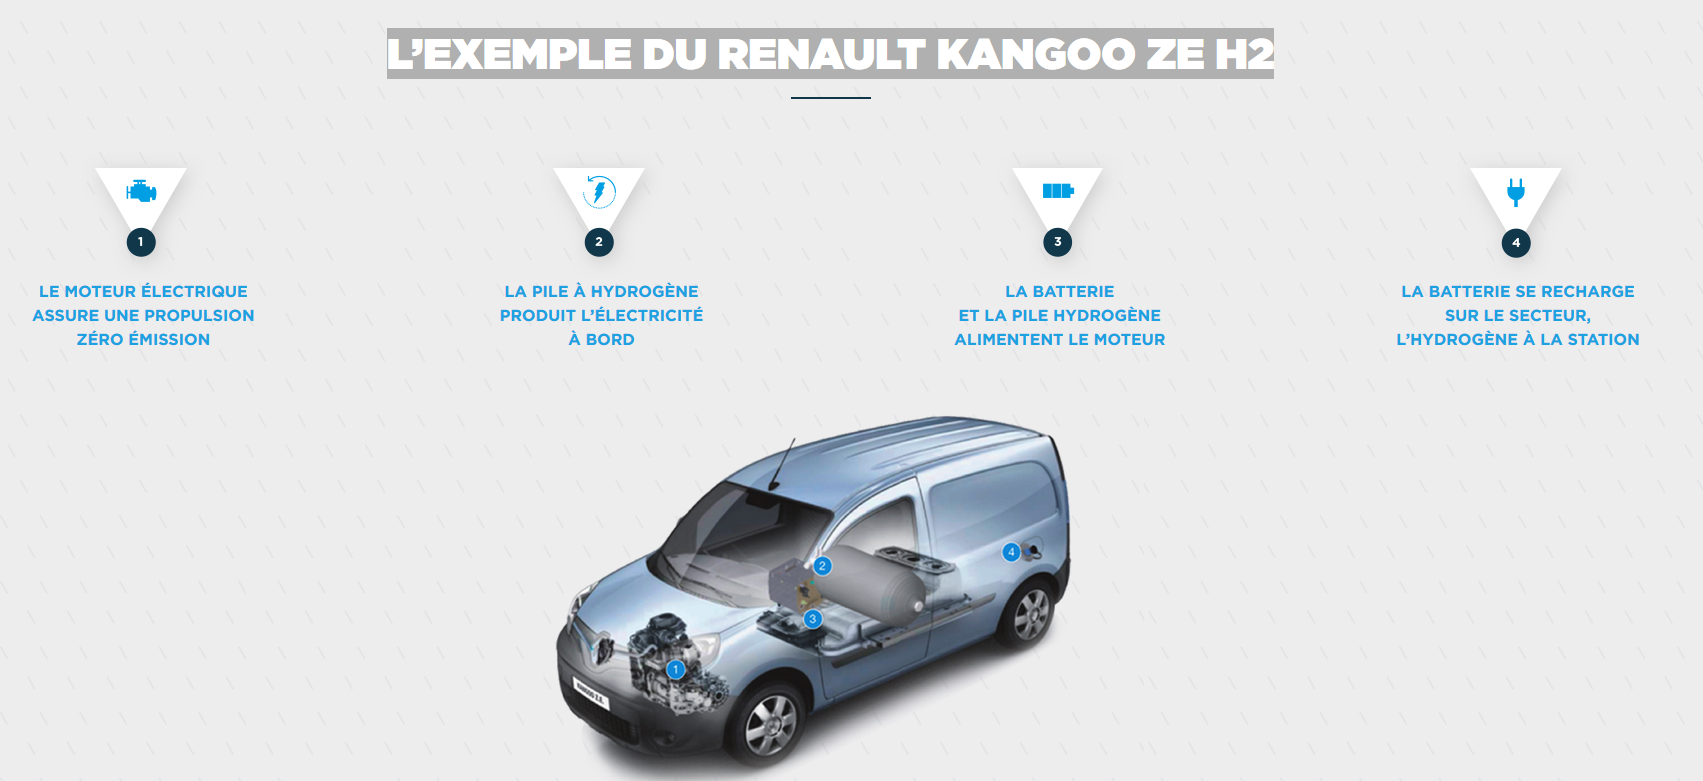
\includegraphics[width=15cm]{images_these/bat.png}}
 	\caption[Une voiture hybride]{Une voiture hybride : véhicule %\href{[https://www.rue89lyon.fr/2014/06/06/teste-le-kangoo-ze-h2-premier-utilitaire-lhydrogene/]}{
 		Kangoo ZE H2 premier utilitaire à l'hydrogène
 		réservoir d'hydrogène de 76 litres (compressé à 350 bars, ce qui nous donne un poids d'environ 1,8kg qu'on recharge en 6 minutes), 27 000 euros : le coût de la pile mais sans la voiture . }%\cite{sitesymbio}
 	\label{vehi}
 \end{figure}
  Par rapport à des modèles 100 \% électriques, ces voitures sont adaptées pour des parcours longue distance. Moins de cinq minutes sont nécessaires pour les recharger et offrir une autonomie de 500 km. A l'usage, elles ne produisent aucune pollution : aucun gaz à effet de serre et aucune particule.
  

 Nous nous intéressons aux véhicules à hydrogène, et, pour mieux les cerner, on s'attarde sur leurs moteurs, leur autonomie, leurs niveaux de pollution, l'étendue de leurs gammes et leurs prix.
 
 Plusieurs types de véhicules peuvent prétendre à l'appellation « véhicule à hydrogène ». On distingue tout d'abord les voitures embarquant une pile à combustible qui utilise de l'énergie cinétique pour alimenter un moteur électrique. Il existe également des modèles avec un moteur à hydrogène qui est alimenté grâce à des réservoirs sous pression stockant de l'hydrogène et fonctionnant sur le même principe qu'un moteur à explosion.
 L'autonomie d'un véhicule à hydrogène dépend principalement de la capacité du réservoir à hydrogène et du rendement de la pile à combustible. Les modèles les plus performants affichent un rendement de l'ordre de 80 \%, permettant d'offrir une autonomie théorique supérieure à 500 kilomètres. À l'heure actuelle, le record est d'ailleurs détenu par la Hyundai Nexo, qui a parcouru 778 kilomètres avec un seul plein.
 L'hydrogène sert à alimenter un moteur électrique.
La voiture à hydrogène ne pollue pas à l'usage car elle ne rejette que de la vapeur d'eau.
 
  En 2020, La gamme de véhicules à hydrogène se limite principalement au Hyundai Nexo, à la Toyota Mirai, au Honda Clarity Fuel Cell et à la Mercedes GLC.
 Non seulement l'offre est limitée, mais les prix restent relativement élevés. A titre d'exemple, la Toyota Mirai coûte au minimum 78 900\euro{}, 60 000\euro{} pour la Honda Clarity Fuel Cell et 53 100\euro{} pour la Mercedes-Benz GLC.
 % Les véhicules à hydrogène sont éligibles à la prime à la conversion (2 500\euro{} ou 5 000\euro{} si achat de moins de 60 000\euro{}) et au bonus écologique (3 000\euro{} ou 6 000\euro{} selon le prix d'achat) en 2020.
 
 En France, dans le secteur des véhicules à hydrogène, la société
 STEP (« Société du Taxi Électrique Parisien ») a lancé en décembre 2015 à Paris la première flotte de taxis composée uniquement de véhicules à hydrogène, sous la marque « hype », en partenariat avec 
 %(site AFHYPAC)\href{[https://www.airliquide.com/fr/science-nouvelles-energies/hydrogene-energie]}{
 Air Liquide. La société française  Symbio FCell est spécialisée dans la conception et la fabrication de systèmes piles à combustible (Il existe une association pour l'hydrogène et les piles à combustible appelée %\href{[http://www.afhypac.org/]} 
 AFHYPAC). Symbio FCell conçoit des kits de pile à hydrogène, pour les véhicules en particulier. Actuellement, Symbio FCell fait du rechargement à moyenne pression (350 bar).
 La meilleure autonomie actuelle sur le marché est 100 km/10 litres d'hydrogène à 700 bars.  A 700 bars l'hydrogène représente trois fois plus de volume que l'essence mais a un rendement deux fois meilleur.
 
 Dans la section suivante, on va lister quelques projets qui participent à la vulgarisation de l'hydrogène.
 \subsection{Liste de projets}

%« Innovative MOBility: Smart and Sustainable Solutions »
Parmi les projets qui mettent en exergue l'hydrogène on peut citer : Hympulsion, ZEV, Blue Hydrogen et PARKOSOL.% et PGMO.

\underline{\textbf{Le projet Hympulsion}} :

Hympulsion a été créé en novembre 2018 par Engie et Michelin pour financer et exploiter vingt \textbf{stations de distribution d'hydrogène} en Auvergne-Rhône-Alpes d'ici à 2023. En 2019 la première station à hydrogène a été installée à Clermont-Ferrand (Voir figure \ref{station_h2}). La région Auvergne-Rhône-Alpes (AURA) participe aussi au développement de l'\textbf{hydrogène} comme vecteur de mobilité décarbonée.

\underline{\textbf{Le projet ZEV}} :

En contrôlant un tiers du capital d'Hympulsion, la région AURA accélère la réalisation du projet Zero Emission Valley (ZEV) qui vise à déployer \textbf{1 000 véhicules à pile à combustible} et \textbf{15 électrolyseurs pour produire de l'hydrogène}.
Ce programme de 50 millions d'euros soutenu par la Banque des territoires et l'Ademe est subventionné à hauteur de 10,1 millions d'euros par l'Union européenne. 
%Les deux premières stations de distribution d'hydrogène seront installées à Chambéry (Savoie) et à Clermont-Ferrand (Puy-de-Dôme).
L'achat de véhicules à pile à combustible sera subventionné proportionnellement au nombre de kilomètres parcourus. ZEV veut propulser la filière hydrogène régionale, qui comprend une centaine d'acteurs, laboratoires, collectivités et entreprises comme McPhy (producteur d'électrolyseur/stockage d'énergie), Symbio FCell (producteur de pile à combustible), Ergosup (producteur d'hydrogène par électrolyse) et Ad-Venta (producteur de systèmes de stockage hydrogène embarqués).


\underline{\textbf{Le projet Blue Hydrogen}} :

Avec sa démarche Blue Hydrogen, Air Liquide s'oriente vers une dé-carbonisation progressive de sa production d'hydrogène dédié aux applications énergétiques.
Concrètement, Air Liquide a pour objectif de produire au moins 50 \% de l'hydrogène nécessaire à ces applications sans rejet de $CO_2$ en combinant :
le reformage de biogaz, 
l'utilisation des énergies renouvelables via l'électrolyse de l'eau et l'usage des technologies de captage et de valorisation du $CO_2$ émis lors de la production d'hydrogène à partir de gaz naturel essentiellement composé de méthane ($CH_4$). \`{A} distance parcourue égale, les voitures électriques à hydrogène permettent de diminuer les émissions de gaz à effet de serre par rapport aux véhicules à combustion.
\begin{figure}[H]
	\centerline{
		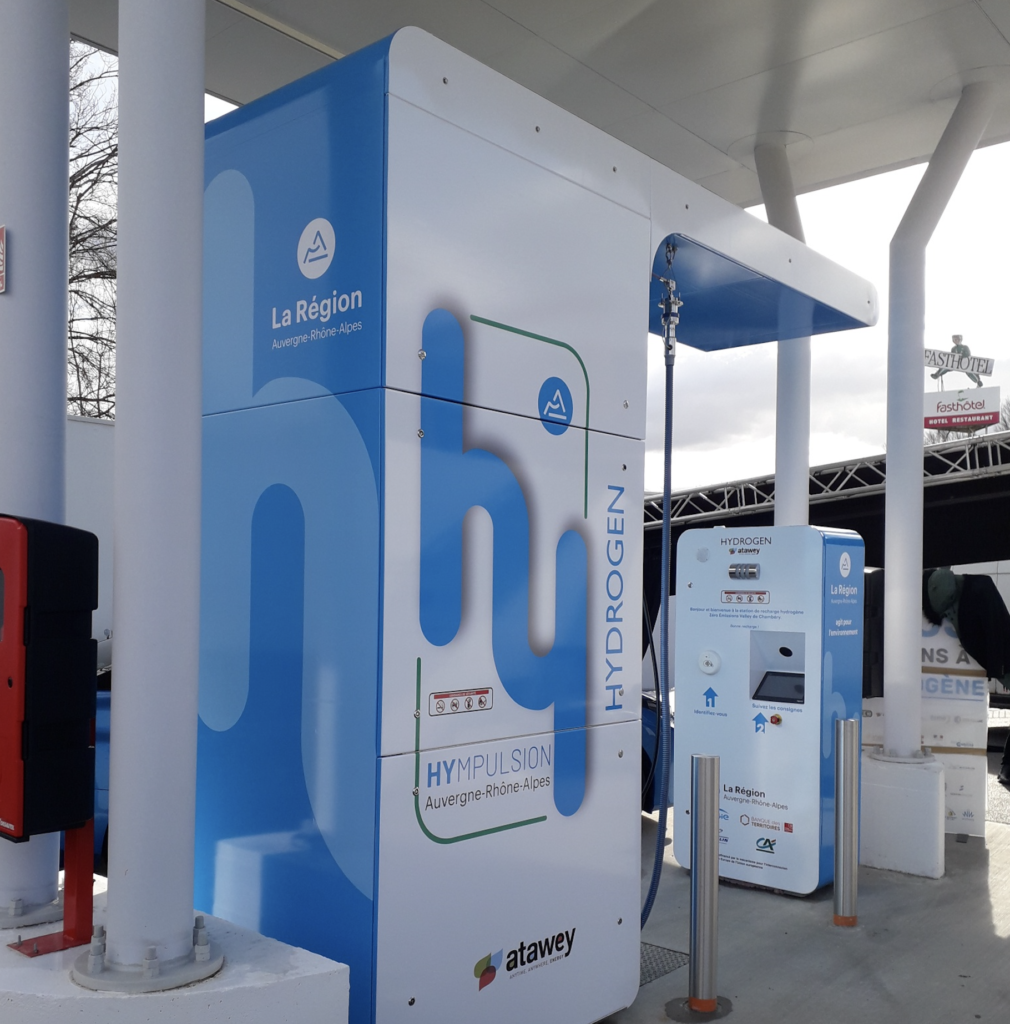
\includegraphics[height=7cm]{images_these/station_h2.png}}
	\caption[Première station à hydrogène de Clermont-Ferrand]{ Première station à hydrogène de Clermont-Ferrand [Rue du Quebec, Zone des Gavranches].}
	\label{station_h2}
\end{figure}


\underline{\textbf{Le projet PARKOSOL}} :

 Engagée dans le développement durable et dans la production locale d'énergie renouvelable, GEG ENeR lance PARKOSOL, un projet portant sur la construction puis l'exploitation de centrales photovoltaïques en ombrières sur des parkings relais de la métropole grenobloise.
L'énergie solaire est une énergie 100\% renouvelable que GEG exploite partout en France et notamment en région Auvergne Rhône-Alpes. GEG ENeR a de nombreux projets de déploiement, de réalisation et d'exploitation d'énergies renouvelables telles que l'hydroélectricité, l'éolien, le biogaz et le photovoltaïque.
Avec PARKOSOL, GEG ENeR veut diminuer les consommations énergétiques, les émissions de gaz à effet de serre et les polluants atmosphériques. Le projet PARKOSOL s'inscrit également dans les démarches de production locale d'énergie renouvelable visées par le plan Air Energie Climat de la collectivité Grenoble Alpes Métropole.

\poubelle{
\underline{\textbf{Le projet PGMO}} :

PGMO est un programme qui a pour but de développer une communauté de recherche autour des thématiques d'optimisation et de recherche opérationnelle. Ils font la recherche sur plusieurs thématiques qui traitent les énergies renouvelables. 
Les acteurs du secteur de l'énergie, comme par exemple EDF ont soutenu la recherche dans le secteur des énergies renouvelable par le biais du Programme Gaspard Monge (PGMO). 
}

\underline{\textbf{Notre projet}} :

Une tendance actuelle du secteur de l'énergie est la décentralisation de la production. Ceci est dû à la fois à la déréglementation des marchés de l'énergie et à l'essor des technologies, qui permettent de plus en plus aux acteurs locaux de devenir de petits producteurs d'énergie (solaire, éolienne, hydrogène, etc ), tout en restant des consommateurs. Ces producteurs/consommateurs locaux peuvent être des usines, des exploitations agricoles et même des particuliers. Cela soulève des questions complexes pour les producteurs d'énergie traditionnels qui, bien qu'ayant perdu leur position monopolistique, restent des acteurs clés, en raison de leur contrôle sur les réseaux de base et les principales centrales hydrauliques et nucléaires.
Dans le cadre des activités du Labex IMOBS3, nous participons à un projet sur la conception et le contrôle d'une micro-usine pour la production d'hydrogène. Cette micro-usine doit fournir aux véhicules autonomes une énergie électrique obtenue à l'aide de piles à combustible à l'hydrogène. Alors que la plupart des productions d'hydrogène sont généralement réalisées par des procédés d'électrolyse coûteux en énergie, les chercheurs s'appuient ici sur l'énergie solaire et la photolyse  \cite{article_hydro_elect_hybrid1}, \cite{Grimes}, qui impliquent une quantité marginale d'énergie électrique externe. Selon ce paradigme, la production/consommation d'énergie devient endogène, et s'effectue selon une sorte de boucle fermée. Il induit un besoin de \textbf{synchronisation} de haut niveau entre les processus de production et de consommation. Pourtant, très peu de travaux abordent la question de la synchronisation des transports  \cite{article_synchro2} et des processus de production d'énergie.


%  \begin{enumerate}
% 	\item Energie ;
%  	\begin{itemize}[label=$\square$]
%		\item Contexte local (PAVIN, Labex)

%  		plateforme Auvergnate pour Véhicules INtelligents) : site expérimental original en France pour le développement de véhicules automatiques en environnement urbain réaliste ;
% 		\item Contexte régional (AURA, filière énergétique nouvelle : airliquide,photovoltaique(grenoble)) ;
%  		\item Contexte international.
%  	\end{itemize}
%  	\item véhicules hybrides.
%  \end{enumerate}

On vient de présenter le contexte et les motivations de ce travail. Dans la section qui suit, on présentera les objectifs de notre projet.
\section{Objectifs de la thèse}
Au cours de ce travail de recherche, on s'est focalisé sur le pilotage \textbf{synchronisé} de la production d'énergie et des activités de services d'une flotte de véhicules.
%Ici, nous laissons de côté la problématique "prévision" qui relève de l'analyse de données , des statistiques et du data mining.
 On se focalise sur le \og décisionnel \fg{}, c'est-à-dire sur la planification synchrone des activités des véhicules d'une part, et de la micro-usine d'autre part. On doit répondre aux questions suivantes :
\begin{itemize}[label=$\square$]
	\item Pour la micro-usine, quand produit-elle de façon à alimenter les véhicules selon leurs besoins énergétiques, au moindre coût?
	\item Pour les véhicules (pour des raisons de simplicité, on se limite à un véhicule), quels parcours suivent-ils ? Quand se rechargent t-ils en carburant ? Et en quelles quantités ?
\end{itemize} 
Nous désignons par \textbf{SMEPC (\textit{Simultaneous Management of Energy Production and Consumption})} notre problème. Le problème \textbf{SMEPC} ainsi posé est spécifique, mais il renvoie à des problématiques générales qui font elles aussi l'objet de l'étude :
\begin{itemize}[label=$\square$]
	\item Une problématique liée à la gestion algorithmique du mécanisme de synchronisation ; %expliquer pourquoi c'est difficile
	\item Une problématique qui est la prise en compte d'une dimension collaborative dans les procédés algorithmique : on a différents acteurs et il faut garder une certaine flexibilité ;
	\item Une problématique de robustesse, liée aux incertitudes sur la production car il nous faut des stratégies adaptés en temps réel.
\end{itemize} 
Ces trois grandes problématiques font parties de l'étude, et elles vont motiver certaines innovations : 
\begin{itemize}[label=$\square$]
	\item Utilisation de la programmation linéaire en nombres entiers pour modéliser notre problème ;
	\item Utilisation du cadre programmation dynamique (DPS : \textit{Dynamic Programming scheme}) pour la gestion des mécanismes de synchronisation ;
	\item Gestion de la dimension collaborative au travers de processus DPS communicants ;
	\item Utilisation des techniques d'apprentissage, plus précisément du \textit{Deep learning}, pour l'approximation des coûts.
	%le traitement des incertitudes et des niveaux décisionnels liés au parcours des véhicules.
\end{itemize} 

La présente contribution porte sur la gestion synchrone  d'une flotte de véhicules électriques équipés de piles à hydrogène, qui sont nécessaires pour effectuer des tâches logistiques locales dans une zone restreinte, et d'une micro-usine chargée de produire le combustible à hydrogène qui sera périodiquement chargé par ces véhicules. Pris dans son ensemble, il comporte simultanément des caractéristiques associées à la prévision, à la sécurité (associée à l'autonomie des véhicules) et à la synchronisation : il faut faire correspondre un calendrier d'enlèvement et de livraison (\textit{Pickup and Delivery} en Anglais) avec la planification de la production ou du stockage d'hydrogène de la micro-usine.

 Ainsi, nous considérons dans cette thèse qu'on a : 
 \begin{itemize}[label=$\square$]
 \item  un seul véhicule utilisé pour effectuer des tâches de livraison. 
 Ce véhicule commence son parcours avec une certaine quantité d'hydrogène, et son réservoir a une capacité limitée. il doit retourner à la micro-usine pour faire le plein. L'ordre de visite des stations ne changera pas.
  
 \item Une micro-usine avec une certaine capacité de stockage, dont la production dépend du rayonnement solaire. 
\end{itemize}
 Notre objectif est de planifier simultanément les opérations de recharge du véhicule et l'activité de production/stockage de la micro-usine.
Pour cela, on doit concevoir des algorithmes et modèles pour planifier la production d'hydrogène par photolyse et la tournée du véhicule. Plus précisément, la planification des opérations de recharge du véhicule consiste à calculer à quelle date le véhicule va se recharger en hydrogène et quelles sont les quantités rechargées à chaque fois. On doit minimiser la durée de la tournée et l'énergie consommée par le véhicule. La planification de l'activité de production/stockage de la micro-usine vise à calculer à quelle date la micro-usine va produire l'hydrogène dont le véhicule aura besoin pour réaliser sa tournée. On doit minimiser les coûts de production en satisfaisant les recharges du véhicule le plus rapidement possible. 

Le problème \textbf{SMEPC} est un nouveau problème. De plus, un point crucial est de concevoir des instances qui seront utiles pour tester numériquement chaque modèle conçu. On explorera aussi la complexité théorique des méthodes de résolution du problème \textbf{SMEPC}.
% Nous nous concentrons ici sur la synchronisation, et ne traitons ni de l'incertitude ni de la conception de l'itinéraire du véhicule. 

Nous allons dans la section suivante présenter brièvement le contenu de chaque chapitre de ce manuscrit. 
\section{Plan de la thèse}
Ce rapport est composé de sept principaux chapitres. On rappelle que dans notre travail, le parcours du véhicule est fixé.

Le \textbf{chapitre} \ref{Etat_art_probleme} fait un état de l'art du problème \textbf{SMEPC} (\textit{Simultaneous Management of Energy Production and Consumption}). On analyse le positionnement de notre problème par rapport aux problèmes de même nature de la littérature. La planification de tournées avec prise en compte de l'énergie pour alimenter les véhicules a été étudiée sous plusieurs formes : problème GVRP (\textit{Green Vehicle Routing Problem}), problème RVRP (\textit{Recharging Vehicle Routing Problem}), problème EVRP (\textit{Electric Vehicle Routing Problem}), problème HVRP (\textit{Hydrogen Vehicle Routing Problem}), problème PRP (\textit{Pollution Routing Problem}). Le problème de planification de la production a été beaucoup étudié et on indique quelques références qui résolvent ce problème. De plus, on s'intéresse aussi aux méthodes de résolution des problèmes de synchronisation qui se rapproche du problème \textbf{SMEPC}. On finit le chapitre \ref{Etat_art_probleme} en présentant le problème IRP (\textit{Inventory Routing Problem}).

Le \textbf{chapitre} \ref{Etat_art_methode} fait un état de l'art des méthodes utilisées pour résoudre le problème \textbf{SMEPC}. Après avoir indiqué brièvement ce qu'est un programme en nombres entiers mixtes, on s'intéresse aux méthodes de résolution par schéma de programmation dynamique ainsi qu'aux méthodes de résolution par heuristique gloutonne. On aborde aussi les méthodes d'apprentissage par réseaux de neurones. Ce chapitre est consacré exclusivement à expliquer ces méthodes et à faire une revue de la littérature des nouvelles techniques qui ont été mises au point dans ces secteurs.
% De plus, on aborde les techniques de gestion des incertitudes dans les problèmes de production.
% puis, présente quelques extensions de ce dernier.

Le \textbf{chapitre} \ref{MIP_3_plus} explique ce qu'est le problème SMEPC. On présente le modèle mathématique du problème \textbf{SMEPC}, et une formulation linéaire mixte MILP (Mixed Integer Linear Programming). Dans ce chapitre nous démontrons aussi que le modèle résultant est NP-Hard. % Mais avant cela on aborde notre problème avec une approche \textit{Branch and Cut}. 
 On présente les procédés de génération des deux paquets instances qu'on nomme INST\_VAR et INST\_CTE. Ce dernier paquet d'instances à été généré à l'aide d'un procédé conçu en 2022 dans le cadre d'un projet de Master réalisé par Alejandro Olivas Gonzalez. 
  Nous finissons ce chapitre en présentant les résultats des expérimentations numériques de nos modèles implémentés sous CPLEX.

Le \textbf{chapitre} \ref{SMEPC_programmation} propose un schéma de programmation dynamique (DPS) désigné par \textbf{DPS\_SMEPC}, proche du schéma de programmation dynamique de \cite{inproceedings-Baptiste-Scheduling}, \cite{article-Demaine-Scheduling}. Ce qui nous permet d'énoncer un schéma d'approximation (\textit{Polynomial Time Approximation Scheme}). Cependant, il s'est avéré que, durant les tests, le DPS tend à impliquer un nombre excessivement élevé d'états. Nous introduisons alors des mécanismes de filtrage :  des mécanismes basés sur la logique, des mécanismes basés sur l'anticipation des incohérences, des mécanismes basés sur la borne supérieure, des mécanismes basés sur le pré-calcul d'une borne inférieure et d'une solution initiale réalisable, et des mécanismes heuristiques, basés sur l'utilisation de mécanismes de dominance faible. Une partie de l'étude est consacrée à l'évaluation de la puissance de filtrage de ces procédés. L'expérimentation numérique vise principalement à évaluer pour le DPS l'impact des différents mécanismes de filtrage et la qualité de l'heuristique de calcul de la borne supérieure.

Le \textbf{chapitre} \ref{Heuristique} se focalise sur la définition d'une heuristique qui résout le problème \textbf{SMEPC}. On désigne par \textbf{Pipe-line VD\_PM} cette heuristique. Les temps de calcul du \textbf{DPS\_SMEPC} augmentent considérablement au fur à mesure que l'instance grossit. De plus, l'algorithme \textbf{DPS\_SMEPC} ne fait pas ressortir la dimension collaborative qui existe entre les sous-problèmes de \textbf{SMEPC}. C'est pour ces raisons qu'on a mis en place une heuristique dont l'objectif est de traiter les instances d'une très grande taille et de faire communiquer deux modules qui traitent chaque sous-problème de \textbf{SMEPC}. Cette heuristique est basée sur un découpage du problème \textbf{SMEPC} en deux problèmes que l'on nomme le \textbf{problème Vehicle-Driver (VD)} et le \textbf{problème Production-Manager (PM)} traités par des schémas de programmation dynamique de façon disjointe dans un premier temps, puis dans un second temps de façon à faire communiquer ces deux problèmes afin d'obtenir une solution du problème \textbf{SMEPC}. Le schéma de programmation dynamique qui résout le problème \textbf{PM} implique un grand nombre d'états, pour cela on va mettre en place des mécanismes de filtrage similaires à ceux du chapitre \ref{SMEPC_programmation} pour limiter ce nombre. On réalise les expérimentations numériques, qui visent principalement à évaluer l'impact des différents mécanismes de filtrage et la qualité de l'heuristique Pipe-line VD\_PM.

%%%%%%!!!!!!!!!!!!!!!!!!!!!!!!!ajouter ceci lorsqu'on ajoutera le dernier chapitre
Le \textbf{chapitre} \ref{neurones} présente des estimateurs de coûts de solutions d'instances du problème \textbf{SMEPC}. Pour faire l'approximation des coûts, on utilise les procédés d'apprentissage appelés réseaux de neurones. On construit des réseaux de neurones basés sur l'architecture Perceptron Multicouche. Le nombre de poids des réseaux de neurones étant élevé, on cherche a les diminuer. Pour cela, on va définir un ensemble d'indicateurs qui permettra de diminuer drastiquement les poids de nos réseaux de neurones.

Pour terminer, le \textbf{chapitre} \ref{conclusion-fin} revient sur l'ensemble des travaux réalisés, notamment l'approche MILP, l'approche programmation dynamique, l'approche heuristique et les résultats expérimentaux obtenus. Un ensemble de perspectives de recherche sont évoquées dans le cadre d'une poursuite de ces travaux. Le premier aspect concerne la planification de la tournée du véhicule, tournée que nous avons supposée fixe dans notre travail. Le second envisage l'incertitude liée à la production d'hydrogène du problème \textbf{SMEPC}. 